
% This LaTeX was auto-generated from MATLAB code.
% To make changes, update the MATLAB code and republish this document.

\documentclass{article}
\usepackage{graphicx}
\usepackage{color}

\sloppy
\definecolor{lightgray}{gray}{0.5}
\setlength{\parindent}{0pt}

\begin{document}

    
    \begin{verbatim}
%  Makes the two graphs called for in HW1, Q1

P_v = 10;
C_s = 0.5;
C_d = 10;
V0 = 30;

P_a = 0:0.5:180;

V_stroke = C_d*P_v - C_s*P_a;

close all
figure
hold on
plot(P_a,V_stroke)
xlabel('P_{arterial} [mmHg]')
ylabel('V_{stroke} [mL]')
grid on
box on
hold off

W_heart = (1.33322e-4) * (P_a - P_v).*(C_d*P_v - C_s*P_a);

figure
hold on
plot(P_a,W_heart)
xlabel('P_{arterial} [mmHg]')
ylabel('W_{heart} [Joules]')
grid on
box on
hold off


%  Now examine a range of C_s

C_s = [0.1, 0.3, 0.5, 0.7];

V_stroke = zeros(4,361);
W_heart  = zeros(4,361);

for i = 1:4
    V_stroke(i,:) = C_d*P_v - C_s(i)*P_a;
    W_heart(i,:)  = (1.33322e-4) * (P_a - P_v).*(C_d*P_v - C_s(i)*P_a);
end

figure
hold on
plot(P_a,V_stroke(1,:),P_a,V_stroke(2,:),P_a,V_stroke(3,:),P_a,V_stroke(4,:))
xlabel('P_{arterial} [mmHg]')
ylabel('V_{stroke} [mL]')
grid on
box on
legend('C_{systolic} = 0.1 mL/mmHg','C_{systolic} = 0.3 mL/mmHg',...
    'C_{systolic} = 0.5 mL/mmHg','C_{systolic} = 0.7 mL/mmHg','location','southwest')
hold off


figure
hold on
plot(P_a,W_heart(1,:),P_a,W_heart(2,:),P_a,W_heart(3,:),P_a,W_heart(4,:))
xlabel('P_{arterial} [mmHg]')
ylabel('W_{heart} [Joules]')
grid on
box on
legend('C_{systolic} = 0.1 mL/mmHg','C_{systolic} = 0.3 mL/mmHg',...
    'C_{systolic} = 0.5 mL/mmHg','C_{systolic} = 0.7 mL/mmHg','location','southwest')
hold off
\end{verbatim}

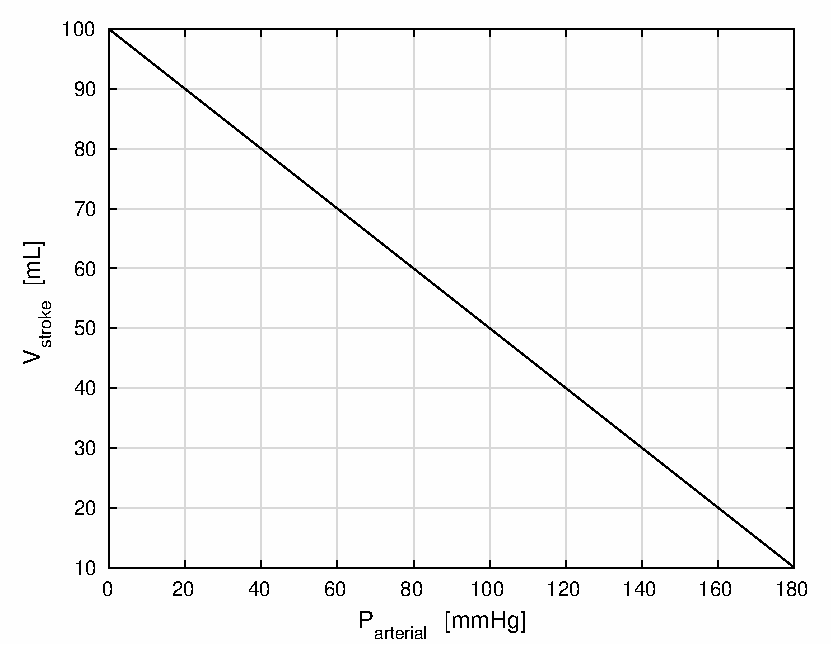
\includegraphics [width=4in]{Q1_01.eps}

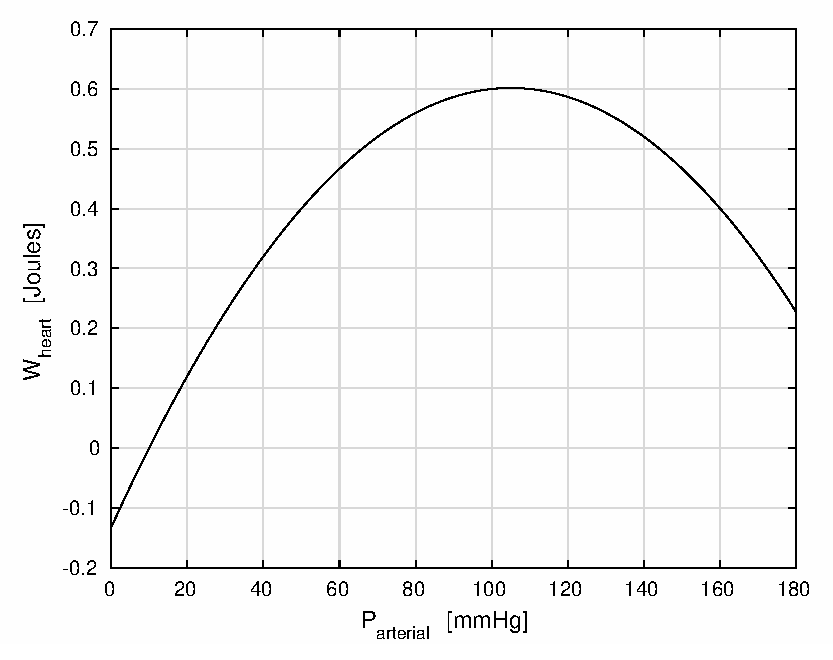
\includegraphics [width=4in]{Q1_02.eps}

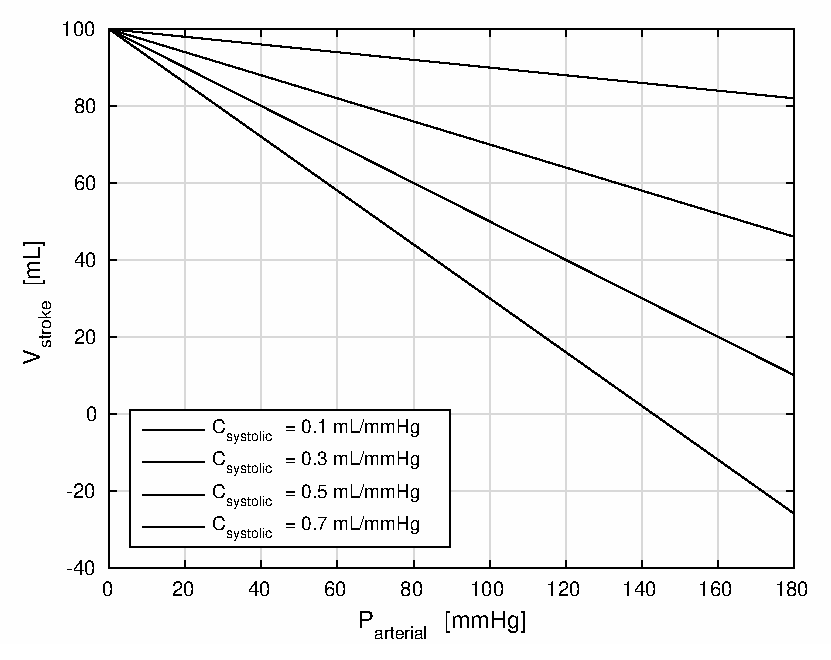
\includegraphics [width=4in]{Q1_03.eps}

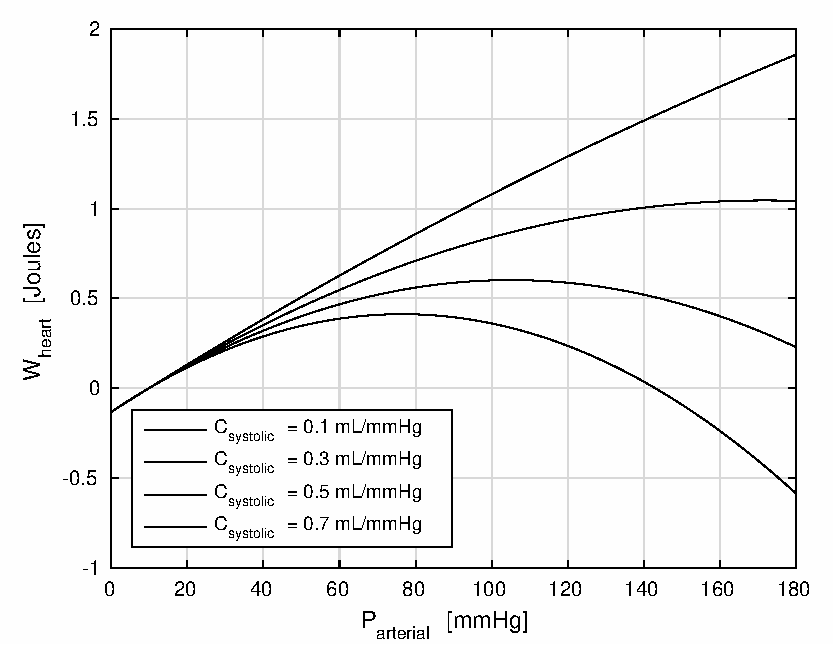
\includegraphics [width=4in]{Q1_04.eps}



\end{document}
    
